\documentclass[11pt]{article}
\usepackage[margin=1.1in]{geometry}
\usepackage{booktabs}
\usepackage{graphicx}
\usepackage[hidelinks]{hyperref}
\usepackage{listings}
\usepackage{xcolor}
\usepackage{pgfplots}
\pgfplotsset{compat=1.18}
\usepackage{placeins} % \FloatBarrier keeps figures inside their section
\usepackage{longtable} % the per-task results table spans pages
\usepackage{caption}   % \captionof for the longtable (not a float)
\lstset{basicstyle=\ttfamily\small, breaklines=true, columns=fullflexible}

% Every number below comes from generated/ — built by `go run ./cmd/bench
% paper <run dirs>` from the committed episode evidence. Do not hand-edit
% figures or tables.
% GENERATED by `bench paper` — do not edit.
\newcommand{\EpisodeCount}{900}
\newcommand{\SemanticPassRate}{50\%}
\newcommand{\RawPassRate}{23\%}
\newcommand{\SemanticPassCount}{150/300}
\newcommand{\RawPassCount}{70/300}
\newcommand{\TaskCount}{20}
\newcommand{\GlmRawPass}{41\%}
\newcommand{\GlmSerenaPass}{49\%}
\newcommand{\GlmSemanticPass}{55\%}
\newcommand{\GptOssRawPass}{5\%}
\newcommand{\GptOssSerenaPass}{36\%}
\newcommand{\GptOssSemanticPass}{54\%}
\newcommand{\QwenRawPass}{24\%}
\newcommand{\QwenSerenaPass}{32\%}
\newcommand{\QwenSemanticPass}{41\%}
\newcommand{\InvalidRawMin}{75\%}
\newcommand{\InvalidRawMax}{86\%}
\newcommand{\InvalidSemanticMax}{2\%}


\title{Compiler-Validated Semantic Editing for Weak Local Coding Models}
\author{Guy J.\ Grigsby\\\small\texttt{guy@grigsby.dev}}
\date{Draft, \today}

\begin{document}
\maketitle

\begin{abstract}
Coding agents edit source code as text. Small locally runnable models
fail at it. Diff formats break, identifiers get guessed, and errors
surface only after files change. \texttt{ago} is a semantic edit
protocol for Go. The agent queries a typechecked workspace and submits
mutations from a versioned operation catalog. The compiler validates
every mutation against an in-memory snapshot before anything reaches
disk. Edits apply as atomic, generation-checked transactions or not at
all. An edit that does not typecheck is unrepresentable, not merely
flagged. Rejections are the conversation. Each one carries typed
diagnostics and paste-ready repairs, the corrected call written out
verbatim. Resending a rejected call unchanged escalates. An oracle
replays each task's ground-truth commit through the protocol before any
model attempts it, so a task enters the benchmark only once it is proven
solvable. Tasks are mined from real commits in traefik, vault, and
boundary. The evaluation is a grid of three modes. One edits files raw.
One addresses symbols through an LSP with advisory validation (Serena).
One sees only the protocol. All run against a frozen engine, so the
benchmark cannot chase the tasks.
% Frozen grid: qwen3.5-9b-udq4 (162906), glm-flash (162855),
% gpt-oss-20b-medium (161639). Numbers below are generated from all three.
Across three locally served models the mode ordering never inverts. The
protocol beats symbol addressing, which beats raw text editing. The
floor 9B model passes \QwenSemanticPass{} of episodes through the
protocol, against \QwenSerenaPass{} with symbol addressing alone and
\QwenRawPass{} raw. The widest gap is the model that is a poor freeform
tool-caller. Its raw pass rate collapses to \GptOssRawPass{}, yet
recovers to \GptOssSemanticPass{} through the protocol. Sampled on-disk
states during editing fail to compile \InvalidRawMin{} to
\InvalidRawMax{} of the time in raw mode, and at most
\InvalidSemanticMax{} in semantic mode, in every model. All code,
per-episode evidence (transcripts, request logs, serving
configurations), and analysis tooling are released.
\end{abstract}

\section{Introduction}
Coding agents edit files as text. A frontier model mostly gets away
with it. A small local model does not. It guesses an identifier that
does not exist, writes a diff that does not apply, or renames in one
file and forgets the other twelve. The error shows up after the bytes
are on disk, when a build breaks, and the agent is already three edits
downstream. The weaker the model, the more of its budget goes to this.

The usual fix is a stricter text format or a bigger model. We take the
opposite position. Keep the small model and change what it is allowed
to do. \texttt{ago} is a semantic edit protocol for Go. The agent does
not write files. It queries a typechecked workspace and submits
mutations from a versioned operation catalog. The compiler checks every
mutation against an in-memory snapshot before anything is written. An
edit that does not typecheck is not caught after the fact. It never
reaches disk.

The catalog is not novel or what guides the models to a solution.
The interaction where the protocol informs the agent's next step is. Every
rejection is a turn in a conversation. It names what is wrong in typed
compiler terms, and it hands back the corrected call, ready to resend.
A weak model does not have to know the fix. It has to be handed the fix
and copy it. That is a much lower bar, and it is the bar most small
models can clear.

We test this against the honest alternatives. The same model, prompts,
and time budget run in three modes. Raw file editing.
LSP symbol addressing with advisory validation (Serena~\cite{serena}).
The protocol. An oracle replays each task's real answer through the
protocol first, so no task enters the benchmark unless it is known to be
solvable. Across three locally served models the ordering never flips.
The protocol beats symbol addressing, which beats raw editing. The gap
is widest for the model that edits text worst. It passes almost nothing
raw and recovers to a majority through the protocol. The reason is
visible mid-edit. In the text modes the workspace fails to compile most
of the time while the agent works. In the protocol it never does.

Our contributions:
\begin{itemize}
\item A semantic, transactional edit protocol for Go where an invalid
edit is unrepresentable, not merely flagged.
\item The rejection-as-repair interaction, and evidence that it is what
lets weak models recover.
\item An oracle that certifies a task is solvable before any model
spends time on it.
\item A three-mode benchmark across three local models, with every
transcript, diff, and score released.
\end{itemize}

\section{Related Work}
Symbol-level agent tooling over LSP navigates semantically but still
edits text, or exposes a single mutation. Serena~\cite{serena} and
gopls's experimental MCP server~\cite{goplsmcp} are examples. The
compiler diagnostics sit right there in those stacks. The difference
here is that validation is not advisory. CODESTRUCT~\cite{codestruct}
frames agents over structured action spaces with syntax-validated
edits, and reports token and accuracy gains. \texttt{ago}'s mutations
are type-checked, transactional, and carry repairs. Repository-scale
editing benchmarks find instructed edits hard for current models
(RES-Q~\cite{resq}, FEA-Bench~\cite{feabench},
EDIT-Bench~\cite{editbench}). Edit-format leaderboards~\cite{aider}
track a separate failure, where a model cannot emit a valid edit in the
required format at all. That is the failure the repair channel converts.
The format stays strict, and the rejection hands back the corrected
call. Compiler-guided patch generation (Repilot~\cite{repilot}) and
typed-hole context (Hazel~\cite{hazel}) take the same
validate-during-generation stance, at expression granularity.

\section{The \texttt{ago} Protocol}
\subsection{Surface}
Ten tools carry a versioned catalog of 33 operations. They span
declaration, statement, test, and project families. Seven query kinds
return deterministic, paged responses. Node handles address statements
inside declarations. Generation counters make staleness explicit
instead of silent.
\subsection{Transactions}
An ordered op list validates as one unit against an in-memory snapshot.
Ops apply to a copy. The dirty set re-typechecks once, in parallel,
scheduled over post-edit import edges. Resolution proofs run, so a
rename that would capture a reference is rejected even though the
compiler would accept it. Then all files write together, or nothing
does. Pre-existing issues in the affected packages are baselined and
tolerated. Real codebases carry history, so only new diagnostics reject.
\subsection{Rejection as conversation}
Every rejection answers one question. What is the correct next call?
It carries typed diagnostics, candidate lists, and
\texttt{possible\_repairs}, complete calls the agent resends verbatim.
Repairs are tested by execution before they are offered. A repair that
would itself reject is worse than none. Resending a rejected call
unchanged escalates. Accepted mutations embed the fresh view of the
touched declaration, so back-to-back edits skip the read round trip.

\section{Oracle Methodology}
Every benchmark task comes from a real commit, so the correct answer is
already known. Before any model attempts a task, the oracle submits
that known answer through the protocol itself. If the right answer
cannot get through, the model never had a chance. The problem is then
ours, whether an engine bug, an extractor error, or a named protocol
ceiling. The task stays out of the roster until it is fixed. This
separates ``the model failed'' from ``the task was impossible'' by
construction. The oracle transcripts are a byproduct, a record of
correct protocol usage for every task.

\section{Benchmark}
Same model, same harness, same prompts, same time cap, three modes.
Token parity across prompts is enforced by test. Raw edits files with
shell tools. Serena addresses symbols through the language server, a
pinned revision of the Serena MCP server, but its validation stays
advisory. Diagnostics are available on request, and nothing blocks a
broken write from landing. Semantic sees only the protocol. The middle
mode is the ablation that separates the two variables the protocol
bundles, symbol addressing and mandatory validation. Scoring is a goal
predicate, a clean typecheck, and scoped tests. The test gate is voided
where a pristine worktree also fails it. Serving is pinned per run.
GLM-4.7-Flash (MoE) runs at UD-Q4\_K\_XL, roughly 20 GiB, with a q8\_0
K/V cache at 128k context. gpt-oss-20b runs at MXFP4, 11.28 GiB of
weights before KV. Qwen3.5-9B runs at UD-Q4\_K\_XL, with its card's
embedding server evicted to fit the larger quant. Serving ran on two
locally hosted GPUs, a 32 GB AMD Radeon AI Pro R9700 and an 8 GB NVIDIA
RTX 3070 Ti, with the harness and typechecking on a separate Apple M5
Max workstation. Per-run hardware and serving configurations are in the
released evidence. Local serving is part of the experiment, constraints
included. Every episode records its
transcript, diff, score, token usage, failure kind, and the daemon's
request log. The evidence is the contribution as much as the numbers.

\subsection{Evaluation freeze}
Every run before the freeze tag is development data. Rejections became
repairs, and oracle failures became engine fixes. That loop is a
contribution, but it cannot also be the headline evidence. The engine
is frozen at a tagged revision (\texttt{eval-freeze-1}). Every episode
records the engine revision it ran under, so the split is auditable.
Headline tables come only from frozen-tag runs over the development set
of 20 oracle-certified tasks. A held-out set mined from etcd, caddy,
and hugo is extracted and certified only after the tag, with the frozen
engine. A certification failure there is reported as a protocol
ceiling, not fixed.

\subsection{Invalid intermediate states}
The mechanism claim is that validation before disk changes what a
repository passes through, not just where an episode ends. A watcher
samples each worktree during the agent's editing window. When the mtime
fingerprint of the Go files changes and then holds still for one
interval, the settled state gets a \texttt{go build ./...} verdict. The
oracle runs as the control and measures the sampler itself. Raw and
advisory modes pass through whatever the model writes. The semantic
mode cannot land a declaration that does not typecheck, so its measured
rate is the write window itself. A mutation touching dozens of call
sites writes files sequentially, and a sample can catch the half-written
state. Replaying every accepted mutation from the flagged episodes
shows each settled state compiles. No host tool wrote Go in any of them.

\section{Results}
Pooled over the frozen grid, semantic passed \SemanticPassCount{}
episodes. Raw passed \RawPassCount{}. The full per-task table
(Appendix~\ref{app:pertask}) tells the sharper story. Raw does best on
the edits a find-and-replace would nearly cover, and drops toward zero
on the tasks that need consistency across files.

\begin{figure}[tbp]
\centering
% GENERATED by `bench paper` — do not edit.
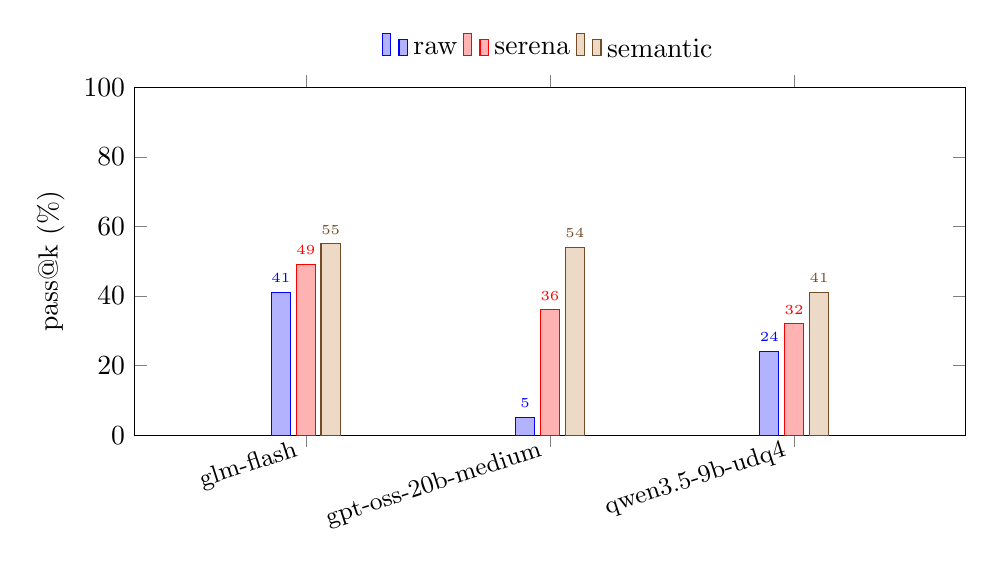
\begin{tikzpicture}
\begin{axis}[
  ybar, bar width=7pt, width=\linewidth, height=6cm,
  ymin=0, ymax=100, ylabel={pass@k (\%)},
  symbolic x coords={glm-flash,gpt-oss-20b-medium,qwen3.5-9b-udq4},
  xtick=data, x tick label style={rotate=18,anchor=east,font=\small},
  legend style={at={(0.5,1.04)},anchor=south,legend columns=-1,draw=none},
  enlarge x limits=0.35, nodes near coords,
  every node near coord/.append style={font=\tiny,/pgf/number format/precision=0,/pgf/number format/fixed},
]
\addplot coordinates {(glm-flash,41) (gpt-oss-20b-medium,5) (qwen3.5-9b-udq4,24)};
\addplot coordinates {(glm-flash,49) (gpt-oss-20b-medium,36) (qwen3.5-9b-udq4,32)};
\addplot coordinates {(glm-flash,55) (gpt-oss-20b-medium,54) (qwen3.5-9b-udq4,41)};
\legend{raw, serena, semantic}
\end{axis}
\end{tikzpicture}

\caption{Pass@k by mode, per model. The ordering semantic $\ge$ serena
$\ge$ raw holds for every model in the grid. The lift is largest where
the model is a weak freeform tool-caller (gpt-oss-20b-medium at
\GptOssRawPass{} raw, \GptOssSemanticPass{} semantic). Generated from
committed episode evidence.}
\label{fig:pass}
\end{figure}

\begin{figure}[tbp]
\centering
% GENERATED by `bench paper` — do not edit.
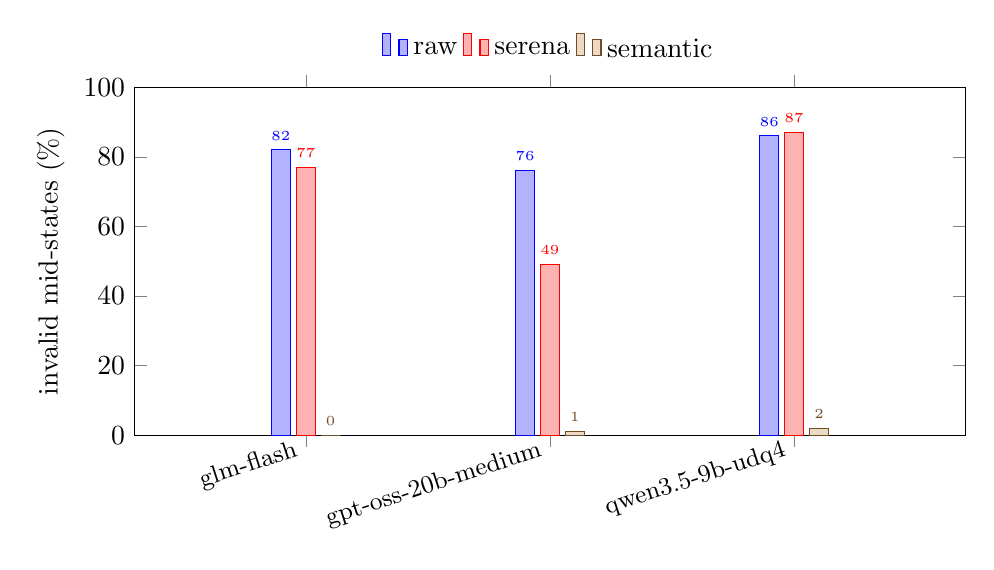
\begin{tikzpicture}
\begin{axis}[
  ybar, bar width=7pt, width=\linewidth, height=6cm,
  ymin=0, ymax=100, ylabel={invalid mid-states (\%)},
  symbolic x coords={glm-flash,gpt-oss-20b-medium,qwen3.5-9b-udq4},
  xtick=data, x tick label style={rotate=18,anchor=east,font=\small},
  legend style={at={(0.5,1.04)},anchor=south,legend columns=-1,draw=none},
  enlarge x limits=0.35, nodes near coords,
  every node near coord/.append style={font=\tiny,/pgf/number format/precision=0,/pgf/number format/fixed},
]
\addplot coordinates {(glm-flash,82) (gpt-oss-20b-medium,76) (qwen3.5-9b-udq4,86)};
\addplot coordinates {(glm-flash,77) (gpt-oss-20b-medium,49) (qwen3.5-9b-udq4,87)};
\addplot coordinates {(glm-flash,0) (gpt-oss-20b-medium,1) (qwen3.5-9b-udq4,2)};
\legend{raw, serena, semantic}
\end{axis}
\end{tikzpicture}

\caption{Fraction of sampled on-disk states that fail \texttt{go build}
during the editing window. The text-editing modes churn through broken
states. The semantic mode cannot land a declaration that does not
typecheck, so its residual is only the multi-file write window.
Generated from the same evidence.}
\label{fig:invalid}
\end{figure}

Two readings stand out. First, the mode ordering
(Figure~\ref{fig:pass}) never inverts across models. Symbol addressing
helps, and mandatory validation helps again on top of it. Second, the
protocol's advantage is not uniform. It is widest for the model that
edits text worst. A strong instruction-follower that is nonetheless a
poor freeform tool user passes almost nothing raw, yet recovers to a
majority through the protocol. The protocol removes exactly the failure
it is prone to. The invalid-intermediate rate (Figure~\ref{fig:invalid})
is the mechanism. Both text modes leave the workspace uncompilable most
of the time mid-edit, while the semantic mode holds it valid throughout.

\FloatBarrier

\section{Limitations}
One language. The protocol is built on Go's type and package model, and
every result here is Go. Whether it helps in a language with a weaker or
slower static checker is untested.

Contamination. The tasks are mined from public repositories the models
have likely trained on. This inflates the absolute pass rates. It is
held equal across all three modes, so the comparison between them is
fair. The claim is the ordering, not the raw percentages.

Small k. Each cell is five episodes, so the per-task confidence
intervals are wide. The result rests on the direction repeating across
twenty tasks and three models, not on any single cell. One quant fixes
each model to a single serving stack. A different quantization or server
could move the numbers.

Narrow task shape. The development set is twenty tasks over a few edit
kinds, rename, add-parameter, and move. These all transform code that
already exists in a known-correct form. Authoring new code is a
different regime. The protocol can still reject an edit that does not
typecheck, but the repair channel has no ground-truth declaration to
hand back, so whether the advantage holds is untested. The held-out set
from etcd, caddy, and hugo widens the task pool, but it does not cross
into authoring. That gap is open.

One baseline per alternative. Raw uses shell tools. Serena is one
symbol-addressing implementation at a pinned revision. A different text
harness or a different LSP server could close or widen the gap.

Uncontrolled conditions. The runs were not executed in a controlled
environment. The hardware is a self-hosted home lab, prosumer and
consumer parts, shared with other load, under thermal and power
conditions that varied across a run.
Rounds were paused and resumed rather than run start to finish, so a
single round spans hours or days of wall clock and whatever the machine
was doing in between. Completed episodes are never re-run on resume, so
the pass counts and invalid-intermediate counts are unaffected. The
timing figures are not. Median time-to-green, the wall-clock seconds to
a passing state, and the cap sit on top of variable generation speed,
and an episode that throttles near
the cap can hit it for a reason that is thermal, not model. This bites
only the episodes already close to the limit, but where a model caps
often it is a real source of noise. Treat the outcome columns as the
result and the timing columns as soft.

Author-run. The serving, harness, and scoring are all ours. Every
transcript, diff, request log, and serving configuration is released so
the result can be checked, but it has not been reproduced independently
yet.

\section{Conclusion}
\texttt{ago} shows that how a weak model edits code matters more than
how big it is. Replace text editing with validated, transactional
mutations. Make every rejection carry its own fix. A 9B model then
becomes a competent repository-scale editor, passing \QwenSemanticPass{}
of episodes through the protocol against \QwenRawPass{} raw. The effect
is largest exactly where it should be, on the model that is worst at
freeform editing, which climbs from \GptOssRawPass{} to
\GptOssSemanticPass{}.

The mechanism is direct. Validation happens before the write, so a
broken state is never on disk for the next step to trip over. The
repair channel turns a rejection into a paste. The model spends its
budget on the task instead of on recovering from its own malformed
edits. The invalid-intermediate rate makes this concrete. The text
modes leave the workspace uncompilable \InvalidRawMin{} to
\InvalidRawMax{} of the time mid-edit. The protocol holds at
\InvalidSemanticMax{} or below.

The scope is narrow and stated. One language. One serving stack per
model. Small k, and the infrastructure is author-run. Contamination is
held equal across modes but still inflates the absolute rates. None of
this moves the ordering, which is the claim, but it caps how far the
absolute numbers travel.

Two things come next. The held-out set from etcd, caddy, and hugo tests
the frozen engine on tasks it was never tuned against. A failure there
is a protocol ceiling we report, not a bug we patch. And the oracle
transcripts record correct protocol usage for every task, a natural
seed for training a model to use it. The protocol that measures a weak
model could also help make one less weak.

\section{Availability}
Code (MIT), all episode evidence, and analysis tooling are at
\url{https://github.com/guygrigsby/agent-go}.

\appendix
\section{Per-task results}
\label{app:pertask}
\captionof{table}{Per-task, per-mode outcomes across the frozen grid.
Generated from committed episode evidence. Each pass@k is over k
episodes. Median time-to-green is over passing episodes.}
\label{tab:results}
{\footnotesize% GENERATED by `bench paper`. Do not edit.
\begin{longtable}{llrrrrr}
\toprule
profile & task & mode & pass@k & median green (s) & capped & resends \\
\midrule
\endhead
\bottomrule
\endlastfoot
glm-flash & boundary\_06d69f69 & raw & 5/5 & 232 & 0 & 0 \\
glm-flash & boundary\_06d69f69 & semantic & 5/5 & 251 & 0 & 2 \\
glm-flash & boundary\_06d69f69 & serena & 5/5 & 175 & 0 & 0 \\
glm-flash & boundary\_35b91c66 & raw & 2/5 & 544 & 3 & 0 \\
glm-flash & boundary\_35b91c66 & semantic & 2/5 & 522 & 3 & 12 \\
glm-flash & boundary\_35b91c66 & serena & 4/5 & 254 & 0 & 0 \\
glm-flash & boundary\_57ffc718 & raw & 0/5 & -- & 5 & 0 \\
glm-flash & boundary\_57ffc718 & semantic & 2/5 & 469 & 3 & 20 \\
glm-flash & boundary\_57ffc718 & serena & 0/5 & -- & 5 & 0 \\
glm-flash & boundary\_687dd1bd & raw & 0/5 & -- & 3 & 0 \\
glm-flash & boundary\_687dd1bd & semantic & 0/5 & -- & 5 & 72 \\
glm-flash & boundary\_687dd1bd & serena & 0/5 & -- & 4 & 0 \\
glm-flash & boundary\_9237d6f7 & raw & 1/5 & 554 & 1 & 0 \\
glm-flash & boundary\_9237d6f7 & semantic & 2/5 & 378 & 1 & 92 \\
glm-flash & boundary\_9237d6f7 & serena & 4/5 & 198 & 0 & 0 \\
glm-flash & boundary\_9354a4eb & raw & 0/5 & -- & 5 & 0 \\
glm-flash & boundary\_9354a4eb & semantic & 0/5 & -- & 5 & 6 \\
glm-flash & boundary\_9354a4eb & serena & 0/5 & -- & 5 & 0 \\
glm-flash & boundary\_9f2c83f3 & raw & 2/5 & 671 & 4 & 0 \\
glm-flash & boundary\_9f2c83f3 & semantic & 4/5 & 354 & 0 & 6 \\
glm-flash & boundary\_9f2c83f3 & serena & 3/5 & 675 & 0 & 0 \\
glm-flash & boundary\_b26814a3 & raw & 1/5 & 720 & 4 & 0 \\
glm-flash & boundary\_b26814a3 & semantic & 3/5 & 720 & 4 & 25 \\
glm-flash & boundary\_b26814a3 & serena & 5/5 & 390 & 0 & 0 \\
glm-flash & boundary\_b4b95e0f & raw & 0/5 & -- & 5 & 0 \\
glm-flash & boundary\_b4b95e0f & semantic & 0/5 & -- & 5 & 4 \\
glm-flash & boundary\_b4b95e0f & serena & 0/5 & -- & 5 & 0 \\
glm-flash & boundary\_bf1486f7 & raw & 0/5 & -- & 5 & 0 \\
glm-flash & boundary\_bf1486f7 & semantic & 4/5 & 657 & 3 & 6 \\
glm-flash & boundary\_bf1486f7 & serena & 0/5 & -- & 5 & 0 \\
glm-flash & boundary\_c0532428 & raw & 5/5 & 449 & 1 & 0 \\
glm-flash & boundary\_c0532428 & semantic & 5/5 & 296 & 0 & 3 \\
glm-flash & boundary\_c0532428 & serena & 5/5 & 156 & 0 & 0 \\
glm-flash & boundary\_caf19f86 & raw & 5/5 & 711 & 2 & 0 \\
glm-flash & boundary\_caf19f86 & semantic & 5/5 & 336 & 0 & 3 \\
glm-flash & boundary\_caf19f86 & serena & 5/5 & 190 & 0 & 0 \\
glm-flash & boundary\_dd2c3807 & raw & 1/5 & 900 & 2 & 0 \\
glm-flash & boundary\_dd2c3807 & semantic & 2/5 & 720 & 5 & 19 \\
glm-flash & boundary\_dd2c3807 & serena & 1/5 & 741 & 3 & 0 \\
glm-flash & boundary\_eb61ac63 & raw & 0/5 & -- & 5 & 0 \\
glm-flash & boundary\_eb61ac63 & semantic & 3/5 & 720 & 5 & 20 \\
glm-flash & boundary\_eb61ac63 & serena & 0/5 & -- & 5 & 0 \\
glm-flash & boundary\_fb1ea92a & raw & 5/5 & 444 & 0 & 0 \\
glm-flash & boundary\_fb1ea92a & semantic & 0/5 & -- & 5 & 76 \\
glm-flash & boundary\_fb1ea92a & serena & 1/5 & 308 & 2 & 0 \\
glm-flash & traefik\_51491463 & raw & 4/5 & 259 & 0 & 0 \\
glm-flash & traefik\_51491463 & semantic & 5/5 & 277 & 0 & 2 \\
glm-flash & traefik\_51491463 & serena & 4/5 & 138 & 0 & 0 \\
glm-flash & vault\_7103bc2c & raw & 0/5 & -- & 2 & 0 \\
glm-flash & vault\_7103bc2c & semantic & 0/5 & -- & 5 & 12 \\
glm-flash & vault\_7103bc2c & serena & 0/5 & -- & 4 & 0 \\
glm-flash & vault\_95b24f55 & raw & 5/5 & 325 & 0 & 0 \\
glm-flash & vault\_95b24f55 & semantic & 5/5 & 367 & 0 & 4 \\
glm-flash & vault\_95b24f55 & serena & 5/5 & 235 & 0 & 0 \\
glm-flash & vault\_caec65a7 & raw & 0/5 & -- & 5 & 0 \\
glm-flash & vault\_caec65a7 & semantic & 5/5 & 422 & 0 & 0 \\
glm-flash & vault\_caec65a7 & serena & 4/5 & 588 & 2 & 0 \\
glm-flash & vault\_cfff8d42 & raw & 5/5 & 349 & 0 & 0 \\
glm-flash & vault\_cfff8d42 & semantic & 3/5 & 720 & 5 & 24 \\
glm-flash & vault\_cfff8d42 & serena & 3/5 & 290 & 3 & 0 \\
gpt-oss-20b-medium & boundary\_06d69f69 & raw & 0/5 & -- & 0 & 0 \\
gpt-oss-20b-medium & boundary\_06d69f69 & semantic & 5/5 & 157 & 0 & 1 \\
gpt-oss-20b-medium & boundary\_06d69f69 & serena & 5/5 & 143 & 0 & 0 \\
gpt-oss-20b-medium & boundary\_35b91c66 & raw & 0/5 & -- & 0 & 0 \\
gpt-oss-20b-medium & boundary\_35b91c66 & semantic & 5/5 & 274 & 0 & 2 \\
gpt-oss-20b-medium & boundary\_35b91c66 & serena & 5/5 & 124 & 0 & 0 \\
gpt-oss-20b-medium & boundary\_57ffc718 & raw & 0/5 & -- & 0 & 0 \\
gpt-oss-20b-medium & boundary\_57ffc718 & semantic & 0/5 & -- & 0 & 6 \\
gpt-oss-20b-medium & boundary\_57ffc718 & serena & 0/5 & -- & 0 & 0 \\
gpt-oss-20b-medium & boundary\_687dd1bd & raw & 0/5 & -- & 0 & 0 \\
gpt-oss-20b-medium & boundary\_687dd1bd & semantic & 0/5 & -- & 0 & 6 \\
gpt-oss-20b-medium & boundary\_687dd1bd & serena & 0/5 & -- & 0 & 0 \\
gpt-oss-20b-medium & boundary\_9237d6f7 & raw & 0/5 & -- & 0 & 0 \\
gpt-oss-20b-medium & boundary\_9237d6f7 & semantic & 4/5 & 331 & 0 & 6 \\
gpt-oss-20b-medium & boundary\_9237d6f7 & serena & 4/5 & 87 & 0 & 0 \\
gpt-oss-20b-medium & boundary\_9354a4eb & raw & 0/5 & -- & 0 & 0 \\
gpt-oss-20b-medium & boundary\_9354a4eb & semantic & 0/5 & -- & 0 & 5 \\
gpt-oss-20b-medium & boundary\_9354a4eb & serena & 0/5 & -- & 0 & 0 \\
gpt-oss-20b-medium & boundary\_9f2c83f3 & raw & 0/5 & -- & 0 & 0 \\
gpt-oss-20b-medium & boundary\_9f2c83f3 & semantic & 4/5 & 275 & 0 & 2 \\
gpt-oss-20b-medium & boundary\_9f2c83f3 & serena & 2/5 & 135 & 0 & 0 \\
gpt-oss-20b-medium & boundary\_b26814a3 & raw & 0/5 & -- & 0 & 0 \\
gpt-oss-20b-medium & boundary\_b26814a3 & semantic & 0/5 & -- & 0 & 5 \\
gpt-oss-20b-medium & boundary\_b26814a3 & serena & 0/5 & -- & 0 & 0 \\
gpt-oss-20b-medium & boundary\_b4b95e0f & raw & 0/5 & -- & 0 & 0 \\
gpt-oss-20b-medium & boundary\_b4b95e0f & semantic & 0/5 & -- & 0 & 6 \\
gpt-oss-20b-medium & boundary\_b4b95e0f & serena & 0/5 & -- & 0 & 0 \\
gpt-oss-20b-medium & boundary\_bf1486f7 & raw & 0/5 & -- & 0 & 0 \\
gpt-oss-20b-medium & boundary\_bf1486f7 & semantic & 3/5 & 160 & 0 & 10 \\
gpt-oss-20b-medium & boundary\_bf1486f7 & serena & 0/5 & -- & 0 & 0 \\
gpt-oss-20b-medium & boundary\_c0532428 & raw & 1/5 & 124 & 0 & 0 \\
gpt-oss-20b-medium & boundary\_c0532428 & semantic & 5/5 & 123 & 0 & 5 \\
gpt-oss-20b-medium & boundary\_c0532428 & serena & 2/5 & 141 & 0 & 0 \\
gpt-oss-20b-medium & boundary\_caf19f86 & raw & 0/5 & -- & 0 & 0 \\
gpt-oss-20b-medium & boundary\_caf19f86 & semantic & 5/5 & 229 & 0 & 0 \\
gpt-oss-20b-medium & boundary\_caf19f86 & serena & 5/5 & 98 & 0 & 0 \\
gpt-oss-20b-medium & boundary\_dd2c3807 & raw & 0/5 & -- & 0 & 0 \\
gpt-oss-20b-medium & boundary\_dd2c3807 & semantic & 0/5 & -- & 0 & 11 \\
gpt-oss-20b-medium & boundary\_dd2c3807 & serena & 0/5 & -- & 0 & 0 \\
gpt-oss-20b-medium & boundary\_eb61ac63 & raw & 0/5 & -- & 0 & 0 \\
gpt-oss-20b-medium & boundary\_eb61ac63 & semantic & 3/5 & 133 & 0 & 0 \\
gpt-oss-20b-medium & boundary\_eb61ac63 & serena & 0/5 & -- & 0 & 0 \\
gpt-oss-20b-medium & boundary\_fb1ea92a & raw & 0/5 & -- & 0 & 0 \\
gpt-oss-20b-medium & boundary\_fb1ea92a & semantic & 0/5 & -- & 0 & 17 \\
gpt-oss-20b-medium & boundary\_fb1ea92a & serena & 0/5 & -- & 0 & 0 \\
gpt-oss-20b-medium & traefik\_51491463 & raw & 0/5 & -- & 0 & 0 \\
gpt-oss-20b-medium & traefik\_51491463 & semantic & 5/5 & 176 & 0 & 8 \\
gpt-oss-20b-medium & traefik\_51491463 & serena & 1/5 & 102 & 0 & 0 \\
gpt-oss-20b-medium & vault\_7103bc2c & raw & 0/5 & -- & 0 & 0 \\
gpt-oss-20b-medium & vault\_7103bc2c & semantic & 0/5 & -- & 0 & 5 \\
gpt-oss-20b-medium & vault\_7103bc2c & serena & 0/5 & -- & 0 & 0 \\
gpt-oss-20b-medium & vault\_95b24f55 & raw & 0/5 & -- & 0 & 0 \\
gpt-oss-20b-medium & vault\_95b24f55 & semantic & 5/5 & 292 & 0 & 1 \\
gpt-oss-20b-medium & vault\_95b24f55 & serena & 5/5 & 174 & 0 & 0 \\
gpt-oss-20b-medium & vault\_caec65a7 & raw & 1/5 & 159 & 0 & 0 \\
gpt-oss-20b-medium & vault\_caec65a7 & semantic & 5/5 & 275 & 0 & 0 \\
gpt-oss-20b-medium & vault\_caec65a7 & serena & 3/5 & 250 & 0 & 0 \\
gpt-oss-20b-medium & vault\_cfff8d42 & raw & 3/5 & 116 & 0 & 0 \\
gpt-oss-20b-medium & vault\_cfff8d42 & semantic & 5/5 & 106 & 0 & 8 \\
gpt-oss-20b-medium & vault\_cfff8d42 & serena & 4/5 & 202 & 0 & 0 \\
qwen3.5-9b-udq4 & boundary\_06d69f69 & raw & 5/5 & 61 & 0 & 0 \\
qwen3.5-9b-udq4 & boundary\_06d69f69 & semantic & 5/5 & 169 & 0 & 0 \\
qwen3.5-9b-udq4 & boundary\_06d69f69 & serena & 5/5 & 92 & 0 & 0 \\
qwen3.5-9b-udq4 & boundary\_35b91c66 & raw & 0/5 & -- & 0 & 0 \\
qwen3.5-9b-udq4 & boundary\_35b91c66 & semantic & 3/5 & 275 & 0 & 2 \\
qwen3.5-9b-udq4 & boundary\_35b91c66 & serena & 3/5 & 142 & 0 & 0 \\
qwen3.5-9b-udq4 & boundary\_57ffc718 & raw & 0/5 & -- & 0 & 0 \\
qwen3.5-9b-udq4 & boundary\_57ffc718 & semantic & 1/5 & 204 & 0 & 3 \\
qwen3.5-9b-udq4 & boundary\_57ffc718 & serena & 0/5 & -- & 1 & 0 \\
qwen3.5-9b-udq4 & boundary\_687dd1bd & raw & 1/5 & 217 & 0 & 0 \\
qwen3.5-9b-udq4 & boundary\_687dd1bd & semantic & 0/5 & -- & 0 & 2 \\
qwen3.5-9b-udq4 & boundary\_687dd1bd & serena & 0/5 & -- & 0 & 0 \\
qwen3.5-9b-udq4 & boundary\_9237d6f7 & raw & 0/5 & -- & 0 & 0 \\
qwen3.5-9b-udq4 & boundary\_9237d6f7 & semantic & 1/5 & 676 & 0 & 2 \\
qwen3.5-9b-udq4 & boundary\_9237d6f7 & serena & 3/5 & 66 & 0 & 0 \\
qwen3.5-9b-udq4 & boundary\_9354a4eb & raw & 0/5 & -- & 0 & 0 \\
qwen3.5-9b-udq4 & boundary\_9354a4eb & semantic & 0/5 & -- & 0 & 4 \\
qwen3.5-9b-udq4 & boundary\_9354a4eb & serena & 0/5 & -- & 0 & 0 \\
qwen3.5-9b-udq4 & boundary\_9f2c83f3 & raw & 0/5 & -- & 0 & 0 \\
qwen3.5-9b-udq4 & boundary\_9f2c83f3 & semantic & 3/5 & 134 & 0 & 3 \\
qwen3.5-9b-udq4 & boundary\_9f2c83f3 & serena & 3/5 & 136 & 1 & 0 \\
qwen3.5-9b-udq4 & boundary\_b26814a3 & raw & 0/5 & -- & 0 & 0 \\
qwen3.5-9b-udq4 & boundary\_b26814a3 & semantic & 2/5 & 204 & 0 & 10 \\
qwen3.5-9b-udq4 & boundary\_b26814a3 & serena & 0/5 & -- & 1 & 0 \\
qwen3.5-9b-udq4 & boundary\_b4b95e0f & raw & 0/5 & -- & 1 & 0 \\
qwen3.5-9b-udq4 & boundary\_b4b95e0f & semantic & 0/5 & -- & 0 & 0 \\
qwen3.5-9b-udq4 & boundary\_b4b95e0f & serena & 0/5 & -- & 0 & 0 \\
qwen3.5-9b-udq4 & boundary\_bf1486f7 & raw & 0/5 & -- & 0 & 0 \\
qwen3.5-9b-udq4 & boundary\_bf1486f7 & semantic & 1/5 & 122 & 0 & 1 \\
qwen3.5-9b-udq4 & boundary\_bf1486f7 & serena & 0/5 & -- & 0 & 0 \\
qwen3.5-9b-udq4 & boundary\_c0532428 & raw & 5/5 & 132 & 0 & 0 \\
qwen3.5-9b-udq4 & boundary\_c0532428 & semantic & 3/5 & 204 & 0 & 17 \\
qwen3.5-9b-udq4 & boundary\_c0532428 & serena & 3/5 & 92 & 0 & 0 \\
qwen3.5-9b-udq4 & boundary\_caf19f86 & raw & 3/5 & 328 & 0 & 0 \\
qwen3.5-9b-udq4 & boundary\_caf19f86 & semantic & 1/5 & 50 & 0 & 5 \\
qwen3.5-9b-udq4 & boundary\_caf19f86 & serena & 4/5 & 98 & 0 & 0 \\
qwen3.5-9b-udq4 & boundary\_dd2c3807 & raw & 0/5 & -- & 0 & 0 \\
qwen3.5-9b-udq4 & boundary\_dd2c3807 & semantic & 3/5 & 166 & 0 & 49 \\
qwen3.5-9b-udq4 & boundary\_dd2c3807 & serena & 0/5 & -- & 0 & 0 \\
qwen3.5-9b-udq4 & boundary\_eb61ac63 & raw & 0/5 & -- & 0 & 0 \\
qwen3.5-9b-udq4 & boundary\_eb61ac63 & semantic & 0/5 & -- & 0 & 15 \\
qwen3.5-9b-udq4 & boundary\_eb61ac63 & serena & 0/5 & -- & 0 & 0 \\
qwen3.5-9b-udq4 & boundary\_fb1ea92a & raw & 0/5 & -- & 0 & 0 \\
qwen3.5-9b-udq4 & boundary\_fb1ea92a & semantic & 0/5 & -- & 0 & 4 \\
qwen3.5-9b-udq4 & boundary\_fb1ea92a & serena & 0/5 & -- & 1 & 0 \\
qwen3.5-9b-udq4 & traefik\_51491463 & raw & 4/5 & 85 & 0 & 0 \\
qwen3.5-9b-udq4 & traefik\_51491463 & semantic & 5/5 & 136 & 0 & 1 \\
qwen3.5-9b-udq4 & traefik\_51491463 & serena & 3/5 & 111 & 0 & 0 \\
qwen3.5-9b-udq4 & vault\_7103bc2c & raw & 0/5 & -- & 0 & 0 \\
qwen3.5-9b-udq4 & vault\_7103bc2c & semantic & 0/5 & -- & 0 & 3 \\
qwen3.5-9b-udq4 & vault\_7103bc2c & serena & 0/5 & -- & 1 & 0 \\
qwen3.5-9b-udq4 & vault\_95b24f55 & raw & 1/5 & 98 & 0 & 0 \\
qwen3.5-9b-udq4 & vault\_95b24f55 & semantic & 5/5 & 274 & 0 & 0 \\
qwen3.5-9b-udq4 & vault\_95b24f55 & serena & 4/5 & 228 & 0 & 0 \\
qwen3.5-9b-udq4 & vault\_caec65a7 & raw & 0/5 & -- & 1 & 0 \\
qwen3.5-9b-udq4 & vault\_caec65a7 & semantic & 5/5 & 590 & 1 & 0 \\
qwen3.5-9b-udq4 & vault\_caec65a7 & serena & 2/5 & 286 & 1 & 0 \\
qwen3.5-9b-udq4 & vault\_cfff8d42 & raw & 5/5 & 60 & 0 & 0 \\
qwen3.5-9b-udq4 & vault\_cfff8d42 & semantic & 3/5 & 291 & 1 & 10 \\
qwen3.5-9b-udq4 & vault\_cfff8d42 & serena & 2/5 & 257 & 0 & 0 \\
\end{longtable}
}

\bibliographystyle{plain}
\bibliography{references}

\end{document}
